\documentclass[11pt]{standalone}
\usepackage{amssymb}
\usepackage{amsmath}
\usepackage[no-math]{fontspec}
\usepackage{unicode-math}
\setmainfont{Libertinus Sans}
\setsansfont{Libertinus Sans}
\setmathfont{Libertinus Math}
\usepackage{pgf,xcolor}
\usepackage{tikz}
\usetikzlibrary{arrows.meta, backgrounds, calc}
\usepackage{pgfplots}
\pgfplotsset{compat=newest}
\usepackage{pifont}

\definecolor{my_darkgray}{HTML}{484949}
\definecolor{my_lightgray}{HTML}{F3F4F4}
\definecolor{my_darkblue}{HTML}{005A94}
\definecolor{my_lightblue}{HTML}{CCDEE9}
\definecolor{my_yellow}{HTML}{FFEC7F}
\definecolor{my_red}{HTML}{E60000}
\definecolor{my_orange}{HTML}{E87846}

\begin{document}
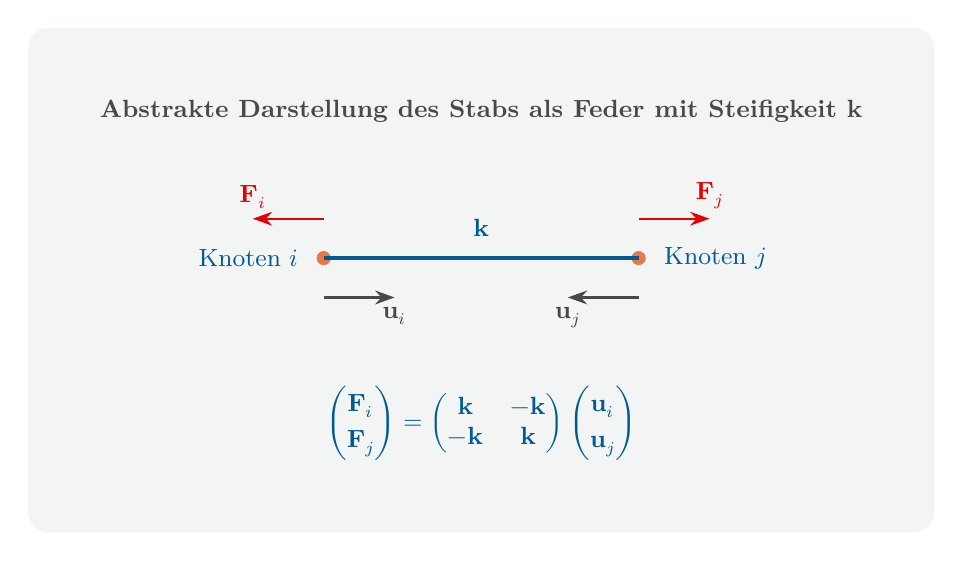
\begin{tikzpicture}[
    show background rectangle,
    background rectangle/.style={fill=my_lightgray, rounded corners=8pt},
    inner frame sep=0.8cm,
    annotation/.style={draw=my_darkgray, thick, -{Stealth[length=7pt, width=5pt]}}
]

    % Knotenpositionen (links: i, rechts: j)
    \coordinate (Ni) at (-2,0);
    \coordinate (Nj) at ( 2,0);

    % Knoten als Punkte
    \draw[fill=my_orange, draw=my_lightgray, thick] (Ni) circle (3pt);
    \draw[fill=my_orange, draw=my_lightgray, thick] (Nj) circle (3pt);

    % Knotenlabels: i links, j rechts
    \node[font=\small, text=my_darkblue, anchor=east]
        at ($(Ni)+(-0.2,0)$) {Knoten $i$};
    \node[font=\small, text=my_darkblue, anchor=west]
        at ($(Nj)+(0.2,0)$) {Knoten $j$};

    % Stab (abstrakte Feder) zwischen den Knoten
    \draw[draw=my_darkblue, ultra thick] (Ni) -- (Nj);

    % Steifigkeit k in der Mitte
    \node[font=\small, text=my_darkblue, anchor=south] at (0,0.15) {$\mathbf{k}$};

    % Verschiebungen u_i und u_j entlang der Stabrichtung (1D-Richtung)
    % u_i: positiv nach rechts
    \draw[annotation]
        ($(Ni)+(0,-0.5)$) -- ($(Ni)+(0.9,-0.5)$);
    \node[font=\small, text=my_darkgray, anchor=north]
        at ($(Ni)+(0.9,-0.5)$) {$\mathbf{u}_i$};

    % u_j: positiv nach links (relativ zu j)
    \draw[annotation]
        ($(Nj)+(0,-0.5)$) -- ($(Nj)+(-0.9,-0.5)$);
    \node[font=\small, text=my_darkgray, anchor=north]
        at ($(Nj)+(-0.9,-0.5)$) {$\mathbf{u}_j$};

    % Kräfte F_i und F_j entlang der Stabrichtung (entgegengesetzt)
    % F_i nach links
    \draw[annotation, draw=my_red]
        ($(Ni)+(0,0.5)$) -- ($(Ni)+(-0.9,0.5)$);
    \node[font=\small, text=my_red, anchor=south]
        at ($(Ni)+(-0.9,0.5)$) {$\mathbf{F}_i$};

    % F_j nach rechts
    \draw[annotation, draw=my_red]
        ($(Nj)+(0,0.5)$) -- ($(Nj)+(0.9,0.5)$);
    \node[font=\small, text=my_red, anchor=south]
        at ($(Nj)+(0.9,0.5)$) {$\mathbf{F}_j$};

    % Kurzer Hinweis auf die Matrixform unten
    \node[font=\small, text=my_darkblue, align=center, anchor=north] at (0,-1.5)
        {$\displaystyle
        \begin{pmatrix}\mathbf{F}_i \\[2pt] \mathbf{F}_j\end{pmatrix}
        =
        \begin{pmatrix}
        \mathbf{k} & -\mathbf{k} \\
        -\mathbf{k} & \mathbf{k}
        \end{pmatrix}
        \begin{pmatrix}\mathbf{u}_i \\[2pt] \mathbf{u}_j\end{pmatrix}$};

    % Titel
    \node[font=\small\bfseries, text=my_darkgray, anchor=south] at (0,1.6)
        {Abstrakte Darstellung des Stabs als Feder mit Steifigkeit $\mathbf{k}$};

\end{tikzpicture}
\end{document}